\section{Our Father's prayer}

This appendix contains texts of Our Father's prayer in different Balto-Slavic languages and Romanian. In non-Slavic ones words with Slavic roots are colored in bold.

\subsection{East Slavic}

\textbf{Russian}

Отче нашъ, сущій на небесахъ!

да святится имя Твое;

да пріидетъ Царствіе Твое;

да будетъ воля Твоя

и на земл\cyryat, какъ на неб\cyryat;

хл\cyryatбъ нашъ насущный дай намъ на сей день;

и прости намъ долги наши,

какъ и мы прощаемъ должникамъ нашимъ;

и не введи насъ в искушеніе,

но избавь насъ от лукаваго.

\textbf{Belorussian}

Ойча наш,

Які ёсць на нябёсах,

няхай свяціцца імя Тваё,

няхай прыйдзе Царства Тваё,

няхай будзе воля Твая

як на небе, так і на зямлі.

Хлеб наш надзённы дай нам сёння;

і даруй нам даўгі нашы,

як і мы даруем даўжнікам нашым;

і не ўвядзі нас у спакусу,

але збаў нас ад злога. 

\textbf{Belorussian (Tarashkevica)}

Ойча наш, каторы ёсьць на небе! 

Сьвяціся Імя Тваё. 

Прыйдзі Валадарства Тваё. 

Будзь воля Твая 

Як у небе, так і на зямлі. 

Хлеба нашага штодзённага 

дай нам сёньня. 

І адпусьці нам грахі нашы, 

як і мы адпускаем 

вінаватым нашым. 

І ня ўводзь нас у спакусу, 

але збаў нас ад злога. 

\textbf{Ukrainian}

Отче наш, що є в небі,
 
нехай святиться ім'я Твоє.

нехай прийде Царство Твоє,

нехай буде воля Твоя,

як на небі, так і на землі;

Хліба нашого щоденного дай нам сьогодні;

й одпусти нам провини наші,

як і ми відпускаємо винуватцям нашим;

і відведи нас від спокуси,

але визволи нас від злого.

\textbf{Rusyn (Podkarpatsky)}

Отче наш, Котрый ись на небесах!

Най сятить ся имня Твоє;

най прийде Царство Твоє;

най буде воля Твоя,

як на небі так и на земли;

хлiб наш насущный дай нам днесь;

и одпусти нам довгы нашы,

як и мы одпущаєме довжникам нашым;

и не введи нас в искушеніє,

но избав нас од лукавого!

\textbf{Rusyn (Pryashôvsky)}

Отче наш, котрый єсь на небесах,

няй святить ся твоє імя,

няй прийде твоє Царьство,

няй ся дїє твоя воля,

як на небі, так і на земли.

Хлїб наш каждоденный дай нам днесь

і одпусть нам нашы довгы,

так як і мы одпущаме своїм довжникам,

і не приведь нас до покушіня,

но ослободь нас од лукавого.

\subsection{West Slavic}

\textbf{Polish}

Ojcze nasz, któryś jest w niebie,

święć się imię Twoje;

przyjdź królestwo Twoje;

bądź wola Twoja,

jako w niebie tak i na ziemi.

Chleba naszego powszedniego daj nam dzisiaj

i odpuść nam nasze winy,

jako i my odpuszczamy naszym winowajcom.

I nie wódź nas na pokuszenie,

ale nas zbaw ode złego.

\textbf{Kashubian}

Òjcze nasz, jaczi jes w niebie,

niech sã swiãcy Twòje miono,

niech przińdze Twòje królestwò,

niech mdze Twòja wòlô

jakno w niebie tak téż na zemi.

Chleba najégò pòwszédnégò dôj nóm dzysô

i òdpùscë nóm naje winë,

jak i më òdpùszcziwómë naszim winowajcóm.

A nie dopùscë na nas pòkùszeniô,

ale nas zbawi òde złégò.

\textbf{Drawänopolabian}

Nôse Wader,

ta toy gis wa Nebisgáy,

Sjungta woarda Tygí Geima,

Tia Rîk komaj,

Tia Willia śčinyôt,

kok wa Nebisgáy,

tôk kak no Zime.

Nôsi wisedanneisna Stgeiba doy nâm dâns,

un wittedoy nâm nôse Ggrêch,

kak moy wittedoyime nôsem Grêsmarim.

Ni bringoy nôs ka Warśikónye,

tay löśoáy nôs wit wisókak Šaudak.

\textbf{Easter Polabian}

Aita Nos,

tâ toi jis wâ nebesai,

Sjęty wordoj Tyji jaimą,

Tyji Rik komaj,

Tyja wyľa mo są ťyńot,

kok wâ nebesai,

tok no zemi,

nosę wisedanesnę sťaibę doj nam dâns,

a wytâdoj nam nose greche,

kok moi wytâdojeme nosim gresnarem.

Ni bringoj nos wâ Warsykongę,

toi losoj nos wyt wisokag šaudag.

\textbf{Silesian}

Uojcze nasz, keryś je we ńebje

bydź pośwjyncůne mjano Twoje;

przińdź krůlestwo Twoje;

bydź wola Twoja

jako we ńebje tak tyż na źymji;

chlyb nasz kożdodźynny dej nům dźiśo;

a uodpuść nům nasze winy,

jako a my uodpuszczůmy naszym wińńikům;

a ńy wůdź nos na pokuszyńy;

nale zbow nos uode złygo.

\textbf{Upper-Sorbian}

Wótče naš, kiž sy w njebjesach.

Swjeć so Twoje mjeno.

Přińdź Twoje kralestwo.

Stań so Twoja wola,

kaž na njebju, tak na zemi.

Wšědny chlěb naš daj nam dźens.

Wodaj nam naše winy,

jako my tež wodawamy swojim winikam.

A njewjedź nas do spytowanja,

ale wumóž nas wot złeho.

\textbf{Lower-Sorbian}

Wóśce nas, kenž sy na njebju,

wuswěśone buź Twójo mě;

pśiź k nam Twójo kralejstwo;

Twója wóla se stań

ako na njebju, tak teke na zemi.

Wšedny klěb naš daj nam źinsa,

a wódaj nam naše winy,

ako my wódawamy swójim winikam.

A njewjeź nas do spytowanja

ale wumóž nas wót togo złego

\textbf{Czech}

Otče náš, jenž jsi na nebesích,

posvěť se jméno tvé,

přijď království tvé,

buď vůle tvá

jako v nebi, tak i na zemi.

Chléb náš vezdejší dejž nám dnes

a odpusť nám naše viny,

jakož i my odpouštíme našim viníkům

a neuveď nás v pokušení,

ale zbav nás od zlého.

\textbf{Slovak}

Otče náš, ktorý si na nebesiach,

posväť sa meno tvoje,

príď kráľovstvo tvoje,

buď vôľa tvoja ako v nebi, tak i na zemi.

Chlieb náš každodenný daj nám dnes

a odpusť nám naše viny,

ako i my odpúšťame svojim vinníkom,

a neuveď nás do pokušenia,

ale zbav nás Zlého.

\subsection{South Slavic}

\textbf{Slovenian}

Oče naš, ki si v nebesih,

posvečeno bodi tvoje ime,

pridi k nam tvoje kraljestvo,

zgodi se tvoja volja 

kakor v nebesih tako na zemlji.

Daj nam danes naš vsakdanji kruh

in odpusti nam naše dolge,

kakor tudi mi odpuščamo svojim dolžnikom,

in ne vpelji nas v skušnjavo, 

temveč reši nas hudega.

\textbf{Serbian}

Оче наш, који си на небесима,

да се свети име Твоје,

да дође царство Твоје;

да буде воља твоја,

и на земљи као на небу.

Хљеб наш насушни дај нам данас,

и опрости нам дугове наше,

као што и ми опраштамо дужницима својим;

и не уведи нас у искушење,

но избави нас од злога.

\textbf{Croatian}

Oče naš,

koji jesi na nebesima, 

sveti se ime Tvoje, 

dođi kraljevstvo Tvoje, 

budi volja Tvoja, 

kako na nebu, tako i na zemlji.

Kruh naš svagdanji daj nam danas, 

i otpusti nam duge naše, 

kako i mi otpuštamo dužnicima našim, 

i ne uvedi nas u napast, 

nego izbavi nas od Zla!. 

\textbf{Bosnian}

Oče naš,

koji jesi na nebesima,

sveti se ime tvoje,

dođi kraljevstvo tvoje,

budi volja tvoja,

kako na nebu tako i na zemlji.

Kruh naš svagdanji daj nam danas,

i otpusti nama duge naše,

kako i mi otpuštamo dužnicima našim,

i ne uvedi nas u napast,

nego izbavi nas od zla.

\textbf{Macedonian}

Оче наш, кој си на небесата,

да се свети името Твое,

да дојде царството Твое,

да биде волјата Твоја,

како на небото, така и на земјата;

лебот наш насушен дај ни го денес

и прости ни ги долговите наши

како и ние што им ги проштеваме на нашите должници;

и не нè воведувај во искушение,

но избави нè од лукавиот.

\textbf{Bulgarian}

Отче наш, Който си на небесата!

Да се свети Твоето име,

да дойде Твоето Царство,

да бъде Твоята воля,

както на небето, тъй и на земята;

Насъщния ни хляб дай ни днес,

и прости нам дълговете ни,

както и ние прощаваме на нашите длъжници,

и не въведи нас в изкушение,

но избави ни от лукавия;

\subsection{Romanian}

Tatăl nostru Care ești în ceruri,

sfințească-se numele Tău,

vie împărăția Ta,

fie voia Ta, precum în cer așa și pe Pământ.

Pâinea noastră cea de toate zilele,

dă-ne-o nouă astăzi

și ne iartă nouă greșalele noastre

precum și noi iertăm greșiților noștri

și nu ne duce pe noi în ispită

ci ne izbăvește de cel rău.

\begin{figure}
	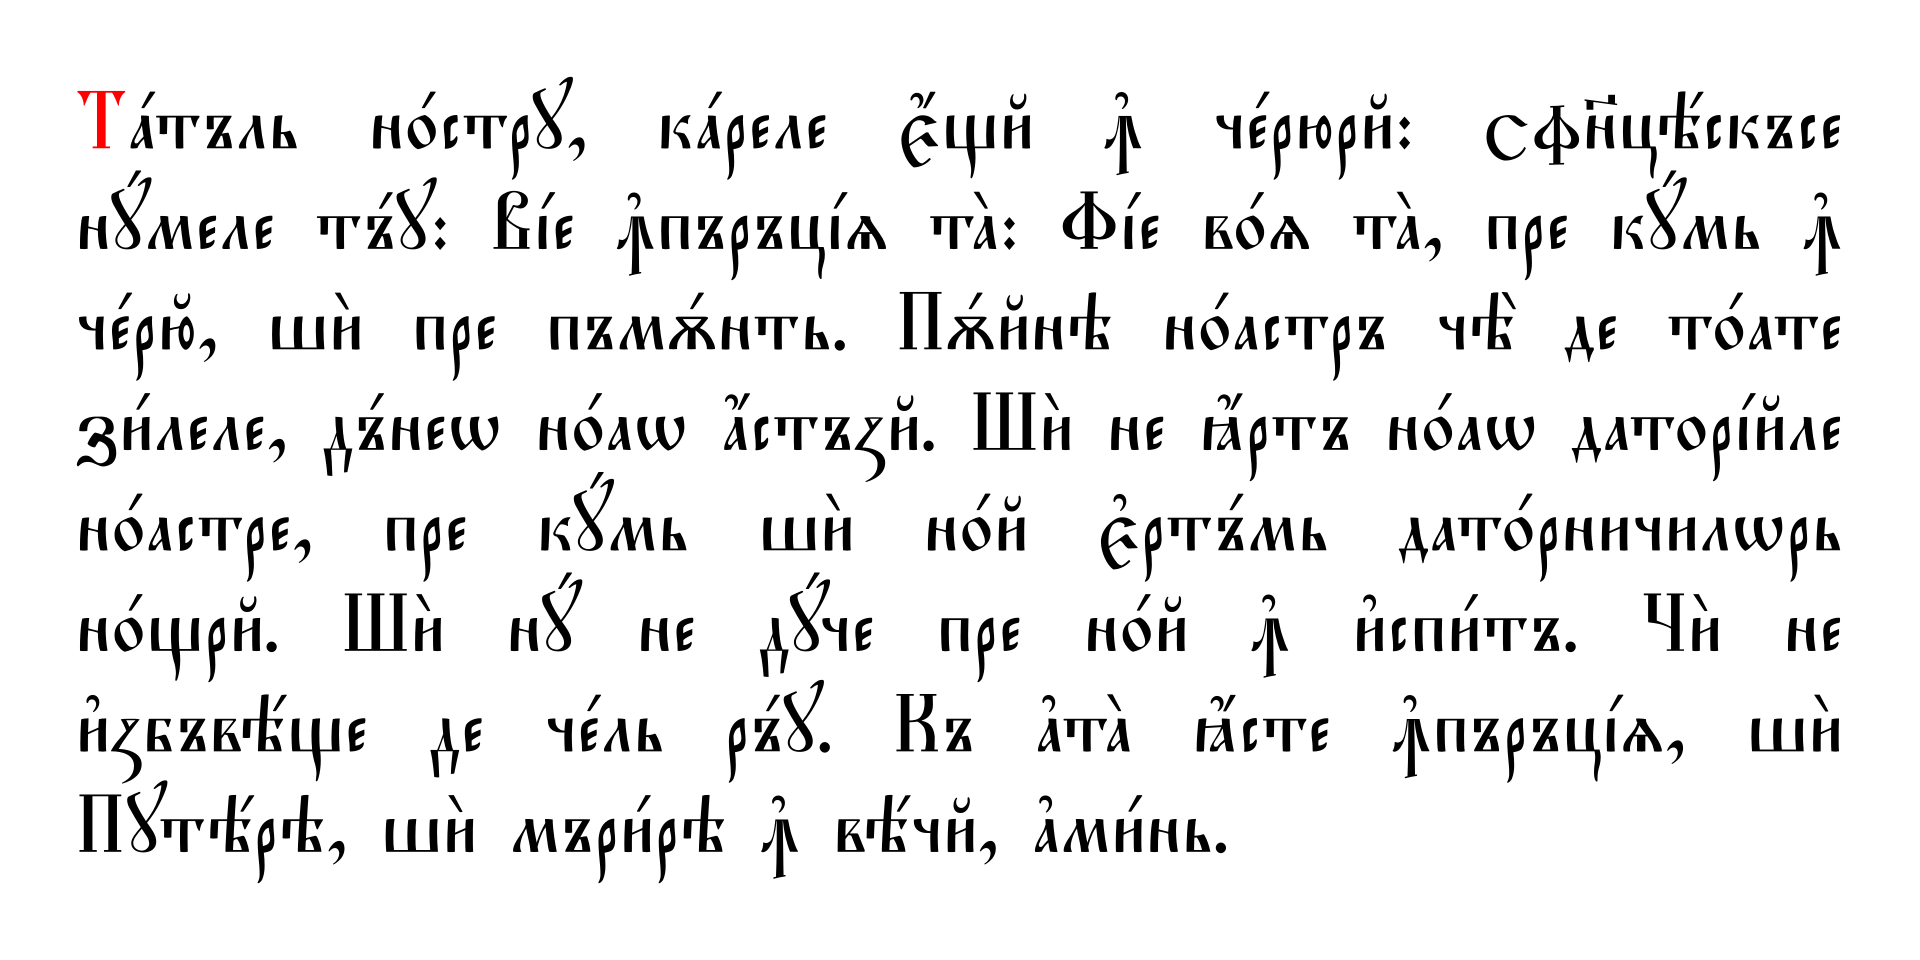
\includegraphics[width=\linewidth]{./sources/of-romanian.png}
	\caption{Our Father's prayer in Romanian}
	\label{fig:of-romanian}
\end{figure}

\subsection{Baltic}

\textbf{Lithuanian}

Tėve mūsų, kuris esi danguje, 

teesie šventas Tavo vardas,

teateinie Tavo karalystė,

teesie Tavo valia

kaip danguje, taip ir žemėje.

Kasdienės mūsų duonos duok mums šiandien

ir atleisk mums mūsų kaltes,

kaip ir mes atleidžiame savo kaltininkams.

Ir nevesk mūsų į pagundą

bet gelbėk mus nuo pikto.

\textbf{Latvian}

Mūsu Tēvs, debesīs,

Svētīts lai top Tavs vārds.

Lai nāk Tava Valstība.

Tavs prāts lai notiek

kā debesīs, tā arī virs zemes.

Mūsu dienišķo maizi dod mums šodien.

Un piedod mums mūsu parādus,

kā arī mēs piedodam saviem parādniekiem.

Un neieved mūs kārdināšanā,

bet atpestī mūs no ļauna.

\textbf{Latgalian}

Tāvs myusu, kas esi debesīs,

svēteits lai tūp Tovs vōrds.

Lai atnōk Tova vaļsteiba.

Tova vaļa lai nūteik, kai debesīs,

tai ari vērs zemes.

Myusu ikdīneiškū maizi dūd mums šudiņ.

Un atlaid mums myusu porōdus,

kai ari mes atlaižam sovim porōdnīkim.

Un naīved myusu kārdynōšonā,

bet izglōb myusus nu ļauna

\textbf{Old Prussian}

Thawe nuson kas tu asse Andangon,

Swintits wirst twais Emmens;

Pergeis twais Laeims;

Twais Quaits audasseisin na Semmey, key Andangon;

Nusan deininan Geittin deis numons schindeinan;

Bha atwerpeis numans nuson Auschautins,

kay mas atwerpimay nuson Auschautenikamans;

Bha ny wedais mans Enperbandan;

Sclait is rankeis mans assa Wargan.

\subsection{Common}

\begin{figure}
	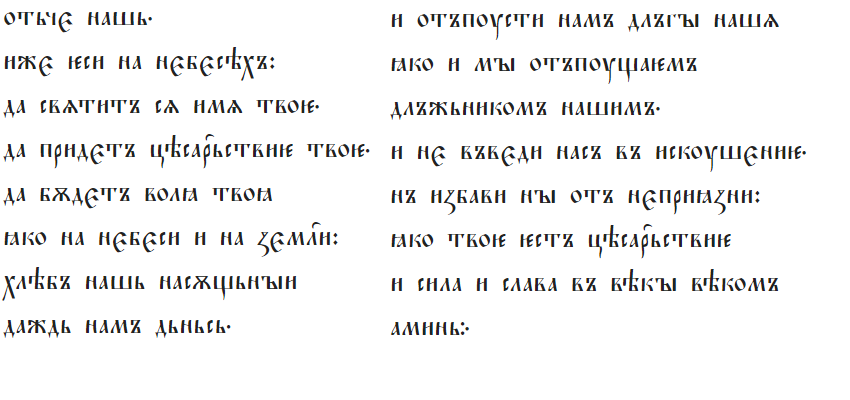
\includegraphics[width=\linewidth]{./sources/of-old-slav.png}
	\caption{Our Father's prayer in Old Slavonic}
	\label{fig:of-old-slav}
\end{figure}

\textbf{Church Slavonic}

Отче наш, Иже еси на небесех!

Да святится имя Твое,

да приидет Царствие Твое,

да будет воля Твоя,

яко на небеси и на земли.

Хлеб наш насущный даждь нам днесь;

и остави нам долги наша,

якоже и мы оставляем должником нашим;

и не введи нас во искушение,

но избави нас от лукаваго.

\begin{figure}
	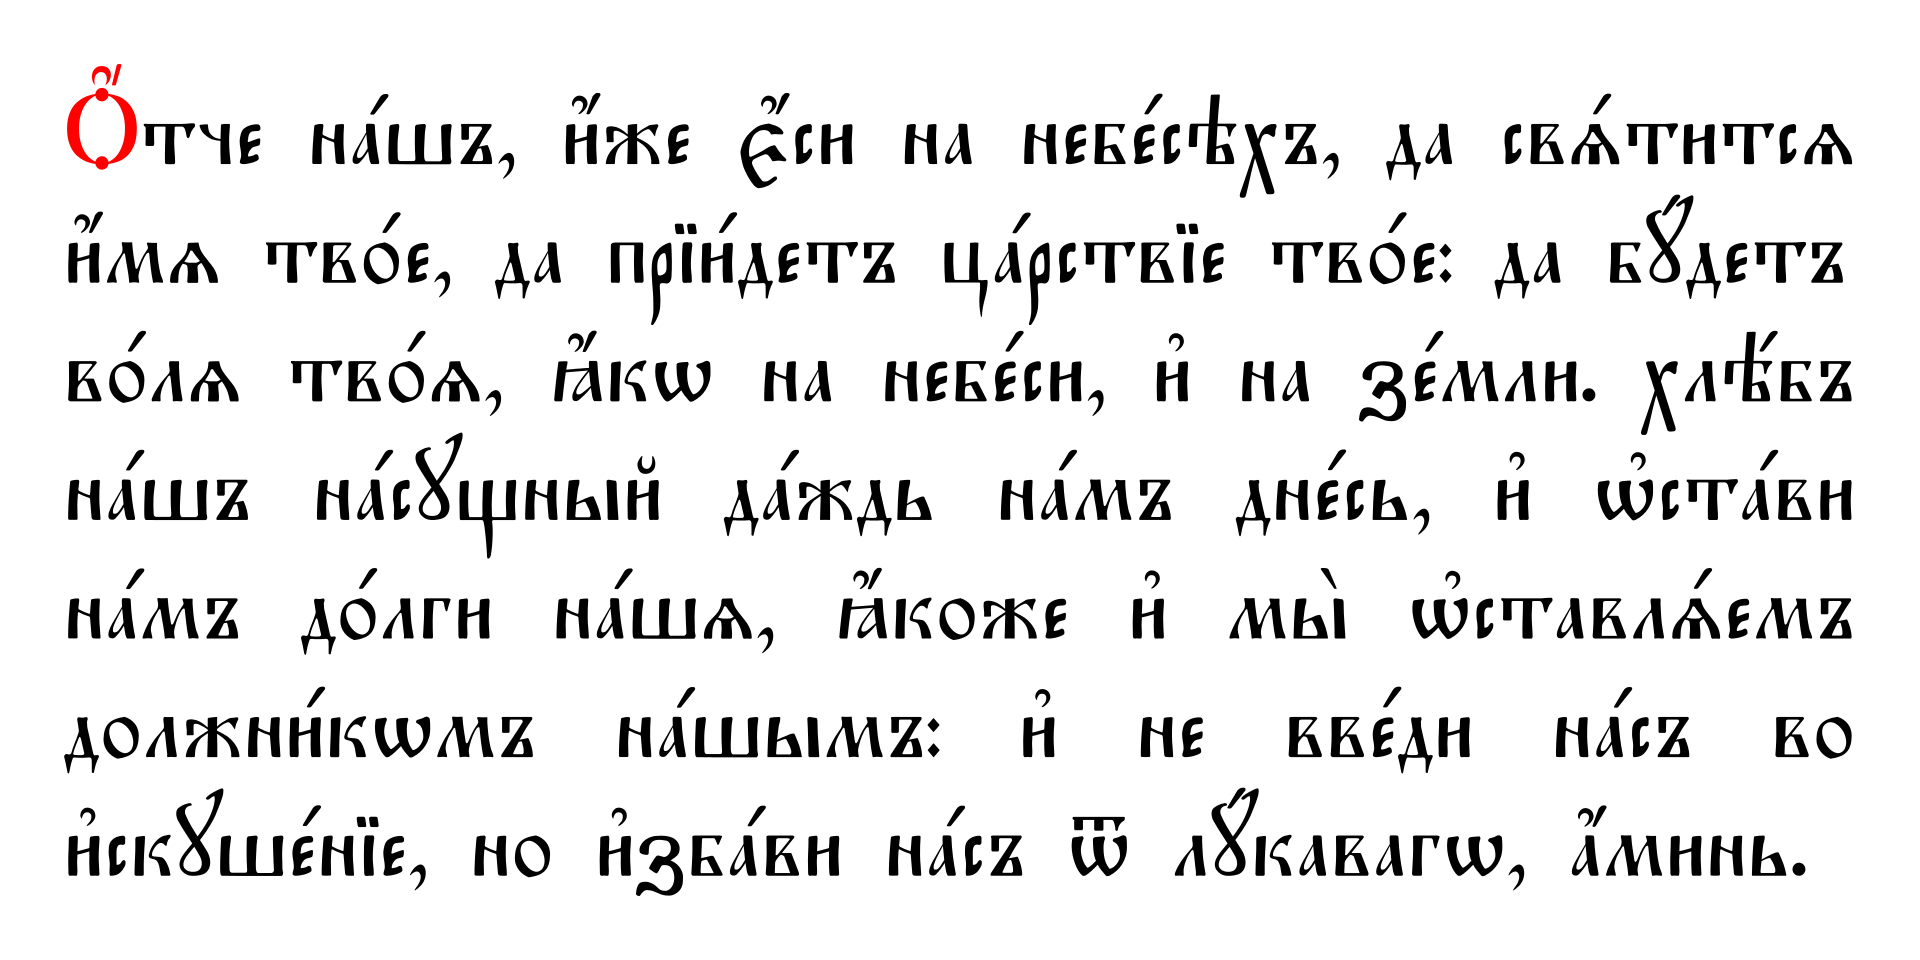
\includegraphics[width=\linewidth]{./sources/of-church-slav.png}
	\caption{Our Father's prayer in Church Slavonic}
	\label{fig:of-church-slav}
\end{figure}

\textbf{Neoslavonic}

Otče naš,

iže jesi na nebesah,

da sveti se ime Tvoje,

da pride cesarstvije Tvoje,

da bude volja Tvoja

jako na nebesi, i na zemlji.

Hlieb naš nasučny daj nam dnes,

i otstav nam dlugy naše,

jako i my otstavujeme dlužnikom našim.

I ne v'vedj nas v napast,

no izbav nas ot lukavego. 

\textbf{Interslavic}

Otče naš, ktory jesi v nebesah,

nehaj svęti sę imę Tvoje.

Nehaj prijde krålevstvo Tvoje,

nehaj bųde volja Tvoja,

kako v nebě tako i na zemji.

Hlěb naš vsjakodenny daj nam dneś,

i odpusti nam naše grěhi,

kako my odpušćajemo našim grěšnikam.

I ne vvedi nas v pokušenje,

ale izbavi nas od zlogo.

\textbf{Novoslovnica}

Otče naš,

Ke jesi na něběsah,

da svęti sę imę Tvoje,

da priǐde cěsarstvo Tvoje,

da bųde volä Tvoja

na zemlï ïsto kako na něbu.

Hlěb naš nasųšten daǐ nam dnësj.

I odpusti nam grěhy našy

Jako že i my odpuštame dòlžnikam našym

I ne vòvëdï nas v izkušenije,

Ale izbavi nas od lųkavoga.
